\chapter{Johdanto}

Kurssin \emph{Tietorakenteet ja algoritmit} tarkoituksena
on opettaa menetelmiä, joiden avulla voimme ratkaista
\emph{tehokkaasti} laskennallisia ongelmia.
Ohjelmoinnin peruskursseilla olemme keskittyneet
ohjelmointitaidon opetteluun.
Nyt on aika siirtyä askel eteenpäin ja alkaa kiinnittää
huomiota myös siihen, miten nopeasti algoritmit toimivat.

Algoritmien tehokkuudella on suuri merkitys käytännössä.
Esimerkiksi netissä toimiva reittiopas on käyttökelpoinen sen vuoksi,
että se antaa meille reitin kuvauksen heti sen jälkeen, kun olemme
ilmoittaneet, mistä mihin haluamme matkustaa.
Jos meidän pitäisi odottaa reitin kuvausta vaikkapa minuutti tai tunti,
tämä rajoittaisi paljon palvelun käyttöä.

Jotta reittiopas toimisi tehokkaasti, sen taustalla on
hyvin suunniteltu algoritmi.
Tällä kurssilla opimme, kuinka voimme luoda itse vastaavia algoritmeja.
Tutustumme kurssilla sekä algoritmien suunnittelun teoriaan että
käytäntöön -- haluamme ymmärtää syvällisesti, mistä algoritmeissa on kysymys,
mutta myös osata toteuttaa niitä käytännössä.

\section{Mitä algoritmit ovat?}

Algoritmi on toimintaohje, jota seuraamalla voimme ratkaista
jonkin laskennallisen ongelman.
Esimerkiksi ''onko luku $n$ alkuluku?'' on laskennallinen ongelma,
jossa algoritmille annetaan \emph{syötteenä} luku $n$
ja sen täytyy ilmoittaa \emph{tulosteena} ''kyllä'' tai ''ei'' riippuen siitä,
onko $n$ alkuluku vai ei.
Esimerkiksi jos algoritmille annetaan luku $7$,
sen täytyy ilmoittaa ''kyllä'',
ja jos algoritmille annetaan luku $12$,
sen täytyy ilmoittaa ''ei''.

Voimme tarkastaa, onko annettu luku $n$ alkuluku, seuraavalla algoritmilla:
käymme läpi kaikki luvut $2,3,\dots,n-1$ ja koetamme
jakaa lukua $n$ jokaisella niistä.
Jos $n$ on jaollinen jollain luvuista, se ei ole alkuluku,
ja muuten se on alkuluku.
Esimerkiksi luku $7$ on alkuluku, koska se ei ole jaollinen
millään luvuista $2,3,\dots,6$,
ja luku $12$ puolestaan ei ole alkuluku, koska $3 \cdot 4 = 12$.
Voimme tutkia tämän algoritmin avulla mistä tahansa luvusta,
onko se alkuluku vai ei.

Algoritmin toiminnan esittämiseen on useita tapoja.
Yksi tapa on selittää sanallisesti, kuinka algoritmi toimii,
kuten teimme äsken.
Toinen tapa taas on antaa koodi, joka toteuttaa algoritmin.
Tällöin meidän täytyy valita jokin ohjelmointikieli,
jonka avulla esitämme algoritmin.
Esimerkiksi voimme tarkastaa seuraavasti Java-kielellä,
onko luku $n$ alkuluku:

\begin{code}
boolean alkuluku = true;
for (int i = 2; i < n; i++) {
    if (n%i == 0) {
        alkuluku = false;
    }
}
\end{code}

Esitämme myös usein algoritmeja \emph{pseudokoodina}
todellisen ohjelmointikielen sijasta.
Tämä tarkoittaa, että kirjoitamme koodia,
joka on lähellä käytössä olevia ohjelmointikieliä, mutta voimme
päättää koodin tarkan syntaksin itse ja ottaa joitakin vapauksia,
joiden ansiosta voimme kuvata algoritmin mukavammin.
Voisimme esimerkiksi esittää äskeisen algoritmin pseudokoodina seuraavasti:

\begin{code}
alkuluku = true
for i = 2 to n-1
    if n%i == 0
        alkuluku = false
\end{code}

Tässä kirjassa esitämme algoritmeja sekä Java-koodina että pseudokoodina
tilanteesta riippuen.
Käytämme Java-koodia silloin, kun haluamme erityisesti kiinnittää huomiota siihen,
miten jokin asia toteutetaan käytännössä Javassa.
Pseudokoodia käytämme taas silloin, kun haluamme kuvata algoritmin yleisen
idean eikä käytetyllä kielellä ole merkitystä.
Taulukko \ref{tab:psekoo} esittää yhteenvedon käyttämämme pseudokoodin syntaksista.

\lstnewenvironment{smallcode}[1][]%
{
   \noindent
   \small
   \minipage{0.47\linewidth} 
   \vspace{0.5\baselineskip}
   \lstset{#1,xleftmargin=0pt}}
{\endminipage}

\begin{table}
\center
\begin{tabular}{ll}
pseudokoodi & Java-koodi \\
\hline
\begin{smallcode}[xleftmargin=0pt]
x = 5
s = "abc"
t = [1,2,3]
\end{smallcode}
&
\begin{smallcode}
int x = 5;
String s = "abc";
int[] t = {1,2,3};
\end{smallcode}
\\
\begin{smallcode}[xleftmargin=0pt]
if a == b
    // koodia
\end{smallcode}
&
\begin{smallcode}
if (a == b) {
    // koodia
}
\end{smallcode}
\\
\begin{smallcode}[xleftmargin=0pt]
while a == b
    // koodia
\end{smallcode}
&
\begin{smallcode}
while (a == b) {
    // koodia
}
\end{smallcode}
\\
\begin{smallcode}[xleftmargin=0pt]
for i = 1 to n
    // koodia
\end{smallcode}
&
\begin{smallcode}
for (int i = 1; i <= n; i++) {
    // koodia
}
\end{smallcode}
\\
\begin{smallcode}[xleftmargin=0pt]
for i = n to 1
    // koodia
\end{smallcode}
&
\begin{smallcode}
for (int i = n; i >= 1; i--) {
    // koodia
}
\end{smallcode}
\\
\begin{smallcode}[xleftmargin=0pt]
sort(x)
\end{smallcode}
&
\begin{smallcode}
Arrays.sort(x);
\end{smallcode}
\\
\begin{smallcode}[xleftmargin=0pt]
print(x)
\end{smallcode}
&
\begin{smallcode}
System.out.println(x);
\end{smallcode}
\\
\begin{smallcode}[xleftmargin=0pt]
swap(a,b)
\end{smallcode}
&
\begin{smallcode}
t = a;
a = b;
b = t;
\end{smallcode}
\\
\begin{smallcode}[xleftmargin=0pt]
a = min(x,y)
b = max(x,y)
\end{smallcode}
&
\begin{smallcode}
a = Math.min(x,y);
b = Math.max(x,y);
\end{smallcode}
\\
\begin{smallcode}[xleftmargin=0pt]
function summa(a,b)
    return a+b
\end{smallcode}
&
\begin{smallcode}
int summa(int a, int b) {
    return a+b;
}
\end{smallcode}
\\
\end{tabular}
\caption{Kirjassa käytetty pseudokoodin syntaksi.}
\label{tab:psekoo}
\end{table}

Ensimmäinen vaihe ohjelmoinnin oppimisessa on oppia
ohjelmoinnin perustaidot niin, että osaamme laatia
\emph{jonkin} toimivan algoritmin annetun ongelman ratkaisemiseen.
On arvokas taito sinänsä, että osaamme ratkaista
ongelman jollakin tavalla.
Toinen vaihe, johon keskitymme tällä kurssilla,
on oppia suunnittelemaan \emph{tehokkaita} algoritmeja.
Tämä tarkoittaa, että haluamme saada aikaan mahdollisuuksien mukaan
jotain parempaa kuin suoraviivaisia
raakaan voimaan perustuvia algoritmeja.

Kiehtova seikka ohjelmoinnissa on, että monimutkaisetkin algoritmit
syntyvät yksinkertaisista aineksista. Keskeiset käsitteet ovat

\begin{itemize}
\item muuttuja, jossa voimme säilyttää tietoa ohjelmassa,
\item ehtolause (\texttt{if}), jonka avulla voimme haarautua ohjelmassa,
\item silmukat (\texttt{for} ja \texttt{while}), joiden avulla voimme
toistaa laskentaa, sekä
\item taulukko, joka on ohjelmoinnin perustietorakenne.
\end{itemize}

Itse asiassa voimme toteuttaa \emph{minkä tahansa} algoritmin
vain näitä aineksia käyttäen.
Tämä on huojentava tieto, koska meidän ei siis tarvitse opetella
suurta määrää ohjelmointikielten ominaisuuksia,
ennen kuin voimme alkaa suunnitella tehokkaita algoritmeja.
Vaikeutena on kuitenkin \emph{keksiä}, kuinka käyttää näitä
tekniikoita eri tilanteessa.

\section{Rekursiiviset algoritmit}

Rekursio on hyödyllinen ohjelmointitekniikka,
joka jää kuitenkin usein sivurooliin ohjelmoinnin perusteiden opiskelussa.
Nyt onkin hyvä hetki perehtyä kunnolla siihen,
mitä hyötyä meille on rekursiosta.
Tulemme tarvitsemaan rekursiota useassa vaiheessa kurssin aikana.

\subsection{Johdatus rekursioon}

Tarkastellaan ensimmäisenä esimerkkinä tehtävää,
jossa haluamme muodostaa kaikki DNA-ketjut,
joiden pituus on $n$.
DNA-ketju on merkkijono, joka muodostuu merkeistä A, C, G ja T.
Esimerkiksi kun $n=3$, ketjut ovat AAA, AAC, AAG, $\dots$, TTC, TTG, TTT.

Voimme ratkaista tehtävän helposti kiinteällä $n$:n arvolla
luomalla $n$ sisäk\-käistä silmukkaa.
Esimerkiksi seuraava koodi vastaa tapausta $n=3$:

\begin{code}
merkit = ["A","C","G","T"]
for i = 0 to 3
    for j = 0 to 3
        for k = 0 to 3
            print(merkit[i]+merkit[j]+merkit[k])
\end{code}

Tämä ratkaisu on toimiva, mutta siinä on yksi ongelma:
kun $n$ muuttuu, niin meidän täytyy muuttaa myös koodia.
Esimerkiksi jos $n=4$, koodista tulee seuraavanlainen:

\begin{code}
merkit = ["A","C","G","T"]
for i = 0 to 3
    for j = 0 to 3
        for k = 0 to 3
            for l = 0 to 3
                print(merkit[i]+merkit[j]+merkit[k]+merkit[l])
\end{code}

Tämä ei ole hyvä ilmiö, vaan haluaisimme saada aikaan \emph{yleisen}
koodin, joka toimisi suoraan millä tahansa $n$:n arvolla.
Rekursio tarjoaa helpon ratkaisun juuri tähän:
pystymme toteuttamaan kätevästi algoritmeja, joissa on
''vaihteleva määrä silmukoita''.

Seuraavassa on rekursiivinen funktio \texttt{muodosta},
joka muodostaa kaikki DNA-ketjut pituutta $n$.
Rekursio lähtee käyntiin, kun parametriksi \texttt{ketju}
annetaan tyhjä merkkijono.
Funktio tarkastaa ensin, onko annettu ketju valmis
eli onko siinä jo $n$ merkkiä.
Jos näin on, funktio tulostaa ketjun eikä tee muuta.
Muussa tapauksessa funktio käy läpi kaikki tavat
lisätä ketjun loppuun seuraava merkki (A, C, G tai T)
ja kutsuu itseään rekursiivisesti jokaisen vaihtoehdon kohdalla.

\begin{code}
function muodosta(ketju)
    if ketju.length() == n
        print(ketju)
    else
        merkit = ["A","C","G","T"]
        for i = 0 to 3
            muodosta(ketju+merkit[i])
\end{code}

\begin{figure}
\center
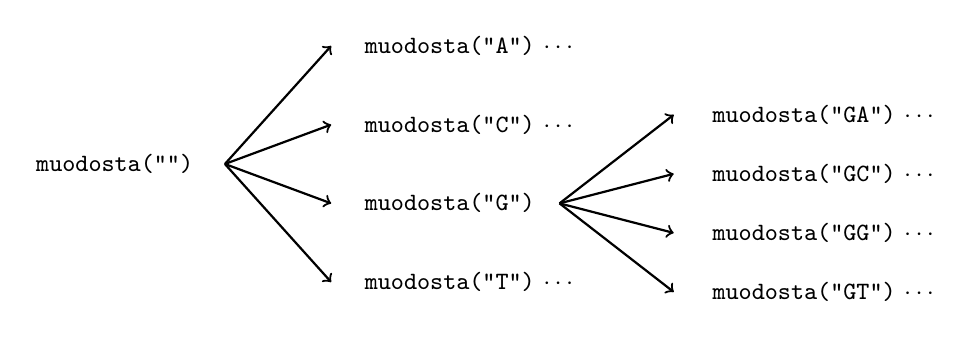
\begin{tikzpicture}[scale=0.5]
\small
\node at (-0.5,0) {\texttt{muodosta("\hspace{0pt}")}};
\node at (8.5,3) {\texttt{muodosta("A")} $\cdots$};
\node at (8.5,1) {\texttt{muodosta("C")} $\cdots$};
\node at (8.5,-1) {\texttt{muodosta("G")} $\phantom{\cdots}$};
\node at (8.5,-3) {\texttt{muodosta("T")} $\cdots$};
\draw[thick,->] (2.3,0) -- (5,3);
\draw[thick,->] (2.3,0) -- (5,1);
\draw[thick,->] (2.3,0) -- (5,-1);
\draw[thick,->] (2.3,0) -- (5,-3);
\node at (17.5,1.25) {\texttt{muodosta("GA")} $\cdots$};
\node at (17.5,-0.25) {\texttt{muodosta("GC")} $\cdots$};
\node at (17.5,-1.75) {\texttt{muodosta("GG")} $\cdots$};
\node at (17.5,-3.25) {\texttt{muodosta("GT")} $\cdots$};
\draw[thick,->] (10.8,-1) -- (13.7,1.25);
\draw[thick,->] (10.8,-1) -- (13.7,-0.25);
\draw[thick,->] (10.8,-1) -- (13.7,-1.75);
\draw[thick,->] (10.8,-1) -- (13.7,-3.25);
\end{tikzpicture}
\caption{DNA-ketjujen muodostaminen rekursiivisesti.}
\label{fig:ketjut}
\end{figure}

Kuva \ref{fig:ketjut} havainnollistaa,
kuinka funktio lähtee muodostamaan ketjuja tyhjästä ketjusta alkaen.
Ensin funktio haarautuu neljään osaan sen mukaan,
onko ketjun ensimmäinen merkki A, C, G vai T.
Tämän jälkeen haarautuminen jatkuu vastaavasti
jokaisessa kutsussa:
esimerkiksi jos ketju alkaa merkillä G,
funktio haarautuu tapauksiin GA, GC, GG ja GT, jne.

\subsection{Osajoukot ja permutaatiot}

Yksi tavallinen rekursion käyttötarkoitus on,
että haluamme käydä läpi kaikki annetun joukon \emph{osajoukot}
eli kaikki tavat valita jokin kokoelma joukon alkioita.
Esimerkiksi joukon $\{1,2,3\}$ osajoukot ovat
$\emptyset$ (tyhjä joukko), $\{1\}$, $\{2\}$, $\{3\}$,
$\{1,2\}$, $\{1,3\}$, $\{2,3\}$ ja $\{1,2,3\}$.
Kun joukossa on $n$ alkioita, osa\-joukkoja on yhteensä $2^n$.

Seuraava rekursiivinen funktio muodostaa joukon
$\{1,2,\dots,n\}$ osajoukot.
Haku lähtee käyntiin, kun kutsumme funktiota
parametrilla $1$.

\begin{code}
function muodosta(x)
    if x == n+1
        // käsittele osajoukko
    else
        valittu[x] = true
        muodosta(x+1)
        valittu[x] = false
        muodosta(x+1)
\end{code}

Ideana on, että parametri $x$ tarkoittaa, minkä alkion
''kohtalon'' ratkaisemme seuraavaksi: joko lisäämme alkion
osajoukkoon tai jätämme sen osa\-joukon ulkopuolelle.
Ensin päätämme, kuuluuko alkio $1$ osajoukkoon vai ei,
sitten toimimme vastaavasti alkion $2$ kohdalla, jne.,
kunnes olemme käsitelleet kaikki $n$ alkiota.
Jokaisen alkion kohdalla merkitsemme päätöksemme taulukkoon
\texttt{valittu} ja jatkamme osajoukon muodostamista rekursiivisesti.
Rekursio päät\-tyy, kun $x=n+1$ eli olemme tehneet valinnan
jokaiselle alkiolle ja olemme saaneet jonkin osajoukon muodostettua.
Tällöin voimme käsitellä muodostetun osajoukon haluamallamme tavalla.
Esimerkiksi voisimme tulostaa osajoukkoon kuuluvat alkiot seuraavasti:

\begin{code}
for i = 1 to n
    if valittu[i]
        print(i)
\end{code}

Tarkastellaan sitten toista tilannetta, jossa haluammekin
muodostaa joukon \emph{permutaatiot}
eli kaikki mahdolliset joukon alkioiden järjestykset.
Esimerkiksi joukon $\{1,2,3\}$ permutaatiot ovat
$(1,2,3)$, $(1,3,2)$, $(2,1,3)$, $(2,3,1)$, $(3,1,2)$ ja $(3,2,1)$.
Kun joukossa on $n$ alkiota, voimme muodostaa siitä yhteensä $n!$ permutaatiota.

Myös permutaatioiden läpikäynti onnistuu kätevästi rekursiolla.
Seuraava rekursiivinen funktio muodostaa joukon $\{1,2,\dots,n\}$ permutaatiot,
kun kutsumme sitä parametrilla $1$.

\begin{code}
muodosta(k)
    if k == n+1
        // käsittele permutaatio
    else
        for i = 1 to n
            if not valittu[i]
                valittu[i] = true
                permutaatio[k] = i
                muodosta(k+1)
                valittu[i] = false
\end{code}

Tässä parametri $k$ tarkoittaa, mihin permutaation kohtaan
valitsemme seuraavaksi alkion.
Aluksi valitsemme alkion kohtaan $1$, sitten
valitsemme alkion kohtaan $2$, jne., kohtaan $n$ asti.
Jokaisessa kohdassa käymme läpi silmukalla kaikki mahdolliset alkiot.
Taulukko \texttt{valittu} kertoo, mitkä alkiot olemme jo valinneet
permutaatioon.
Jos alkio $i$ ei ole vielä mukana permutaatiossa, haaraudumme tapaukseen,
jossa valitsemme sen kohtaan $k$ ja merkitsemme tämän tiedon
taulukkoon \texttt{permutaatio}.
Lopulta kun $k=n+1$, olemme saaneet muodostettua jonkin permutaation
ja rekursiivinen haarautuminen päättyy.
Tällöin voimme käsitellä permutaation haluamallamme tavalla,
esimerkiksi tulostaa alkioiden järjestyksen seuraavasti:

\begin{code}
for i = 1 to n
    print(permutaatio[i])
\end{code}

\subsection{Peruuttava haku}

\emph{Peruuttava haku} on yleinen rekursiivinen menetelmä,
jota käyttäen voimme muodostaa järjestelmällisesti
kaikki ratkaisut annettuun ongelmaan.
Ideana on aloittaa tyhjästä ratkaisusta ja käydä
joka askeleella läpi rekursiivisesti kaikki mahdolliset tavat,
kuinka voimme laajentaa ratkaisua.

Peruuttava haku on raa'an voiman menetelmä,
ja voimme käyttää sitä vain silloin,
kun ratkaisujen määrä on niin pieni,
että ehdimme käydä läpi kaikki ratkaisut.
Kuitenkin jos voimme käyttää peruuttavaa hakua,
se on mainio tekniikka,
koska voimme olla varmoja, että oikein toteutettu
peruuttava haku löytää kaikki ratkaisut.

\begin{figure}
\center
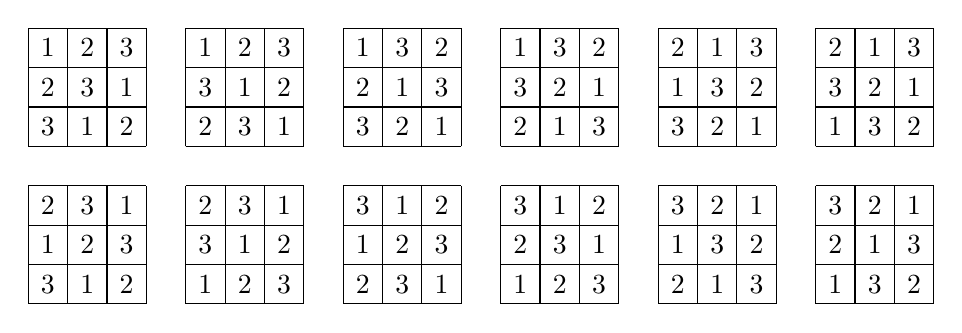
\begin{tikzpicture}[scale=0.5]
\newcommand\nelio[9]{
\draw (0,0) grid (3,3);
\foreach \x/\y/\v in {0/0/#1,1/0/#2,2/0/#3,0/1/#4,1/1/#5,2/1/#6,0/2/#7,1/2/#8,2/2/#9} \node at (0.5+\x,2.5-\y) {\v};
}
\begin{scope}
\nelio{1}{2}{3}{2}{3}{1}{3}{1}{2}
\end{scope}
\begin{scope}[xshift=4cm]
\nelio{1}{2}{3}{3}{1}{2}{2}{3}{1}
\end{scope}
\begin{scope}[xshift=8cm]
\nelio{1}{3}{2}{2}{1}{3}{3}{2}{1}
\end{scope}
\begin{scope}[xshift=12cm]
\nelio{1}{3}{2}{3}{2}{1}{2}{1}{3}
\end{scope}
\begin{scope}[xshift=16cm]
\nelio{2}{1}{3}{1}{3}{2}{3}{2}{1}
\end{scope}
\begin{scope}[xshift=20cm]
\nelio{2}{1}{3}{3}{2}{1}{1}{3}{2}
\end{scope}
\begin{scope}[yshift=-4cm]
\nelio{2}{3}{1}{1}{2}{3}{3}{1}{2}
\end{scope}
\begin{scope}[yshift=-4cm,xshift=4cm]
\nelio{2}{3}{1}{3}{1}{2}{1}{2}{3}
\end{scope}
\begin{scope}[yshift=-4cm,xshift=8cm]
\nelio{3}{1}{2}{1}{2}{3}{2}{3}{1}
\end{scope}
\begin{scope}[yshift=-4cm,xshift=12cm]
\nelio{3}{1}{2}{2}{3}{1}{1}{2}{3}
\end{scope}
\begin{scope}[yshift=-4cm,xshift=16cm]
\nelio{3}{2}{1}{1}{3}{2}{2}{1}{3}
\end{scope}
\begin{scope}[yshift=-4cm,xshift=20cm]
\nelio{3}{2}{1}{2}{1}{3}{1}{3}{2}
\end{scope}
\end{tikzpicture}
\caption{Kaikki 12 latinalaista neliötä kokoa $3 \times 3$.}
\label{fig:latnel}
\end{figure}

Tarkastellaan esimerkkinä tehtävää, jossa haluamme käydä läpi
kaikki kokoa $n \times n$ olevat \emph{latinalaiset neliöt}
eli ruudukot, joissa kullakin vaaka- ja pystyrivillä
esiintyy tarkalleen kerran jokainen luku $1,2,\dots,n$.
Kyseessä on siis yksinkertaistus tutusta sudoku-tehtävästä.
Esimerkiksi kuva \ref{fig:latnel} näyttää kaikki 12 latinalaista neliötä kokoa $3 \times 3$.

Toteutamme peruuttavan haun niin, että valitsemme joka askeleella
ruudukon kohtaan $(y,x)$ tulevan luvun.
Numeroimme ruudukon vaaka- ja pystyrivit kokonaisluvuin $1,2,\dots,n$.
Aloitamme haun ruudukon vasemmasta yläkul\-masta ja etenemme
rivi kerrallaan alaspäin.
Seuraava rekursiivinen algoritmi toteuttaa haun,
kun sitä kutsutaan parametreilla $(1,1)$:

\begin{code}
muodosta(y,x)
    if y == n+1
        // käsittele ratkaisu
    else if x == n+1
        muodosta(y+1,1)
    else
        for i = 1 to n
            if not vaaka[y][i] and not pysty[x][i]
                vaaka[y][i] = pysty[x][i] = true
                nelio[y][x] = i
                muodosta(y,x+1)
                vaaka[y][i] = pysty[x][i] = false
\end{code}

Algoritmin alussa on kaksi erikoistapausta:
jos $y=n+1$, olemme saaneet muodostettua
yhden latinalaisen neliön.
Jos taas $x=n+1$, olemme saaneet jonkin vaakarivin
valmiiksi ja alamme muodostaa seuraavaa vaakariviä.
Muuten kyseessä on perustapaus, jossa haluamme
valita kohtaan $(y,x)$ tulevan luvun.
Käymme läpi kaikki mahdolliset tavat for-silmukalla,
jossa $i$ on valittava luku.
Koska jokainen luku saa esiintyä vain kerran kullakin
vaaka- ja pystyrivillä, käytämme kahta aputaulukkoa:
$\texttt{vaaka}[y][i]$ kertoo, onko vaakarivillä $y$
jo lukua $i$, ja vastaavasti $\texttt{pysty}[x][i]$ kertoo,
onko pystyrivillä $x$ jo lukua $i$.
Jos voimme sijoittaa luvun $i$ kohtaan $(y,x)$,
merkitsemme tämän taulukkoon $\texttt{nelio}[y][x]$
ja lisäksi päivitämme taulukoita $\texttt{vaaka}$ ja $\texttt{pysty}$.
Sitten jatkamme hakua rekursiivisesti seuraavaan
oikealla olevaan ruutuun.

\begin{table}
\center
\begin{tabular}{rr}
ruudukon koko $n$ & neliöiden määrä \\
\hline
1 & 1 \\
2 & 2 \\
3 & 12 \\
4 & 576 \\
5 & 161280 \\
6 & 812851200 \\
\end{tabular}
\caption{Latinalaisten neliöiden määrät, kun $n=1,2,\dots,6$.}
\label{tab:latnel}
\end{table}

Kun olemme saaneet muodostettua latinalaisen neliön, voimme käsitellä
sen haluamallamme tavalla, kuten tulostaa neliön sisältö
taulukon \texttt{nelio} perusteella
tai vain laskea, montako neliötä on olemassa.
Taulukko \ref{tab:latnel} listaa latinalaisten neliöiden
määrät arvoilla $n=1,2,\dots,6$, jotka pystymme laskemaan
nopeasti tässä esitetyn algoritmin avulla.
Suuremmilla $n$:n arvoilla haku alkaa kestää liian kauan
ja meidän tulisi keksiä keino tehostaa hakua,
jos haluaisimme laskea määriä suuremmissa tapauksissa.

\section{Matemaattinen tausta}

Tietorakenteiden ja algoritmien teoria perustuu matematiikkaan,
ja käym\-me kirjassa pikkuhiljaa läpi tarvittavia tietoja.
Seuraavassa on joitakin merkintöjä ja käsitteitä, joista on hyötyä
useassa kirjan kohdassa.

\subsection{Summakaavat}

Voimme laskea lukujen $1,2,\dots,n$ summan kaavalla
\[1+2+\dots+n = \frac{n(n+1)}{2}.\]
Esimerkiksi
\[1+2+3+4+5 = \frac{5 \cdot 6}{2}=15.\]
Kaavan voi ymmärtää niin, että laskemme yhteen $n$ lukua,
joiden suuruus on \emph{keskimäärin} $(n+1)/2$.

Toinen hyödyllinen kaava on
\[2^0+2^1+\dots+2^n = 2^{n+1}-1.\]
Esimerkiksi
\[1+2+4+8+16=32-1.\]
Tässä voimme ajatella, että aloitamme luvusta $2^n$
ja lisäämme siihen aina puolet pienemmän luvun lukuun $1$ asti.
Tämän seurauksena pääsemme yhtä vaille lukuun $2^{n+1}$ asti.

Esitämme joskus summia merkinnän $\sum$ avulla.
Siinä on ideana antaa muuttujan ala- ja yläraja sekä
joka askeleella summaan lisättävä arvo.
Esimerkiksi voimme merkitä
\[1^2 + 2^2 + \dots + n^2 = \sum_{i=1}^n i^2.\]

Tämä merkintä on itse asiassa hyvin lähellä ohjelmoinnin
for-silmukkaa, koska seuraava koodi ajaa saman asian:

\begin{code}
summa = 0
for i = 1 to n
    summa += i*i
\end{code}

\subsection{Logaritmit}

Logaritmin määritelmän mukaan $\log_b n =x$
tarkalleen silloin kun $b^x=n$.
Esimerkiksi $\log_2 32=5$, koska $2^5=32$.

Algoritmiikassa logaritmin kantaluku $b$ on usein 2,
ja voimme ajatella, että logaritmi kertoo, montako kertaa
meidän täytyy \emph{puolittaa} luku $n$, ennen kuin pääsemme lukuun 1.
Esimerkiksi $\log_2 32 =5$, koska tarvitsemme 5 puolitusta:
\[32 \rightarrow 16 \rightarrow 8 \rightarrow 4 \rightarrow 2 \rightarrow 1\]
Tässä kirjassa oletamme, että logaritmin kantaluku on 2,
jos ei ole toisin mainittu,
eli voimme kirjoittaa lyhyesti $\log 32 = 5$.

Logaritmeille pätee kaavat
\[\log_b(x \cdot y) = \log_b(x)+\log_b(y)\]
ja
\[\log_b(x / y) = \log_b(x)-\log_b(y).\]
Ylemmästä kaavasta seuraa myös
\[\log_b(x^k) = k \log_b(x).\]
Lisäksi voimme vaihtaa logaritmin kantalukua kaavalla
\[\log_u(x) = \frac{\log_b(x)}{\log_b(u)}.\]